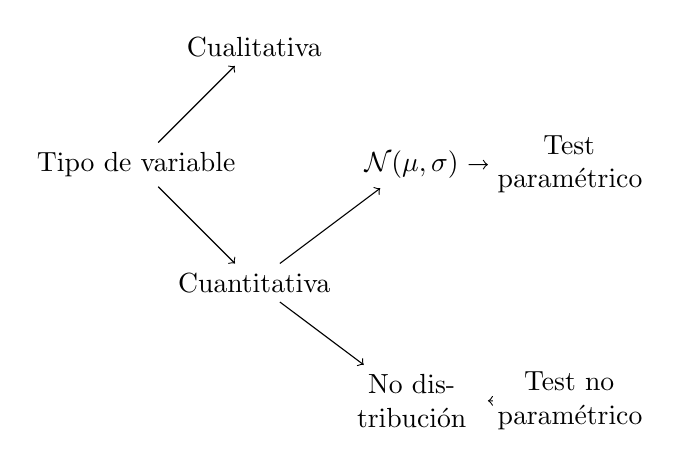
\begin{tikzpicture}
\node {Tipo de variable} [grow'=right, ->]
   child {node {Cualitativa}
         }
   child[missing] {node {}}
   child {node {Cuantitativa}
            child [level distance=2cm] {node {$\mathcal{N}(\mu,\sigma)$}
                     {child [level distance=2cm] {node {\parbox[c]{12ex}{\centering Test param\'etrico}}}}
                  }
            child[missing] {node {}}
            child [level distance=2cm] {node {\parbox[c]{12ex}{\centering No distribuci\'on }}
                     {child [level distance=2cm] {node {\parbox[c]{12ex}{\centering Test no param\'etrico}}}}
                  }
         } ;

\end{tikzpicture}
